\documentclass[11pt,a4paper,oneside,oldfontcommands]{ctexart}
\usepackage{tabularx}
\usepackage{array}
\usepackage{bm}
\usepackage{hyperref}
\usepackage{graphicx}
\usepackage{amsmath}
\usepackage{algorithm}
\usepackage{algpseudocode}
\usepackage{fancyhdr}
\pagestyle{fancy}

\hypersetup{hypertex=true,
	colorlinks=true,
	linkcolor=red,
	anchorcolor=blue,
	citecolor=blue}
\fancyhf{}
\chead{\textbf{算法设计与分析}}
\fancyhead[r]{\bfseries\thepage}
\fancyhead[l]{\bfseries\rightmark}
\renewcommand{\headrulewidth}{0.4pt} % 注意不用 \setlength
\renewcommand{\footrulewidth}{0pt}

\floatname{algorithm}{算法}
\renewcommand{\algorithmicrequire}{\textbf{输入:}}
\renewcommand{\algorithmicensure}{\textbf{输出:}}

\begin{titlepage}
	\title{\Huge\textbf{算法设计与分析 作业四}\\}
	\author{\Large\textbf{作者}:吴润泽 \and{\Large\textbf{学号}:181860109}\\
	\\
	\and {\Large\textbf{Email}:\href{mailto:181860109@smail.nju.edu.cn}{181860109@smail.nju.edu.cn}}\\}
	\date{\Large\today}
\end{titlepage}
\begin{document}
\maketitle
\newpage
\tableofcontents
\cleardoublepage
\section*{Chapter 4}
\markright{Chapter 4}
\addcontentsline{toc}{section}{Chapter 4}
{\subsection*{problem 4.2}}
\markright{problem 4.2}
\addcontentsline{toc}{subsection}{problem 4.2}
\hypertarget{(1)}{\subsubsection*{(1)}}
\textbf{$\Rightarrow$}如果w是v在DFS树中的后继结点,那么$actice(w)\subseteq active(v)$:\\
当$w\ne v$时,
因为w是v的后继节点,所以$v.discover<w.discover$,并且$v.finish>w.finish$。所以$actice(w)\subset active(v)$。当$w=v$时显然成立。
\textbf{$\Leftarrow$}如果$actice(w)\subseteq active(v)$,那么w是v在DFS树中的后继结点:\\
当$w\ne v$时,因为$active(w)\subseteq active(v)$,即$v.discover<w.discover$,并且$v.finish>w.finish$,即在遍历v的过程中将w遍历,即w是v的后继结点。
\hypertarget{(2)}{\subsubsection*{(2)}}
由\hyperref[(1)]{(1)}可知,w不是v的后继结点$\Leftrightarrow actice(w)\not\subset active(v)$。
v不是w的后继结点$\Leftrightarrow actice(v)\not\subset active(w)$得证。
\subsubsection*{(3)}
\paragraph*{\textcircled{1}}
\textbf{$\Rightarrow$}如果vw是CE,那么v和w没有祖先和后继关系,
由\hyperref[(2)]{(2)}可知active(w)和active(v)互不包含。同时CE说明在v指向w时,w已经是黑色节点,w已经遍历结束,
所以active(w)在active(v)之前。\\
\hspace*{20pt}\textbf{$\Leftarrow$ }active(w)在active(v)之前,w先完成整个遍历过程,后才遍历到v。且二者没有祖先后继关系,
那么边vw即为CE。\\
\paragraph*{\textcircled{2}}
\textbf{$\Rightarrow$}vw是DE,即v指向w时w为黑色,并且$active(w)\subset active(v)$,
若不存在第三个节点x,满足x是v的后继,w是x的后继,则v遍历到w时w一定为白色,边为TE。
即一定有$active(w)\subset active(x)\subset active(v)$。\\
\hspace*{20pt}\textbf{$\Leftarrow$}如果存在结点x,满足$active(w)\subset active(x)\subset active(v)$,
由\hyperref[(1)]{(1)}可知,x是v的后继,w是x的后继,且在遍历时v先走到x,然后x走到w,即v是w的祖先结点,因此vw是DE。\\
\paragraph*{\textcircled{3}}
\textbf{$\Rightarrow$}vw是TE,即v指向w时w为白色,w是v的后继,由\hyperref[(1)]{(1)}可知,$active(w)\subset active(v)$。
若存在x,满足$active(w)\subset active(x)\subset active(v)$,则在遍历时v先走到x,然后x走到w,
那么v是w的祖先而非父结点,与vw是TE矛盾。\\
\hspace*{20pt}\textbf{$\Leftarrow$}同理可得w是v的后继,且v直接指向w,则w是白色,即vw是TE。\\
\paragraph*{\textcircled{4}}
vw是BE$\Leftrightarrow$v是w的后继$\Leftrightarrow active(v)\subset active(w)$得证。\\

{\subsection*{problem 4.5}}
\markright{problem 4.5}
\addcontentsline{toc}{subsection}{problem 4.5}
\noindent \hypertarget{1.}{1. }不可能是TE。如果是TE,则有$active(v)\subset actice(u)$,即$v.finishTime>u.discoverTime$,故不成立。\\
2. 不可能是BE。如果是BE,则有$active(u)\subset actice(v)$,即$v.finishTime>u.discoverTime$,故不成立。\\
3. 不可能是DE。如果是DE,同样的v是u的后继结点,满足$active(v)\subset actice(u)$,同\hyperref[1.]{1.}不成立。\\
4. 可能是CE。
x结点先遍历v,然后从v返回x,x遍历u,易知$v.finishTime<u.discoverTime$。\\
如图所示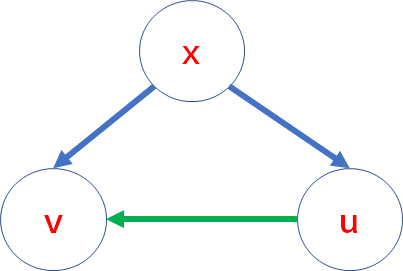
\includegraphics{CEORDER.png}\\
\newpage
{\subsection*{problem 4.7}}
\markright{problem 4.7}
\addcontentsline{toc}{subsection}{problem 4.7}
在第一次DFS中,将结点压栈,同一强连通片的源头结点是最后一个压栈的。\textbf{(引理4.4)}若l是某个强连通片首节点,x是另一个强连通片中的节点,
并且存在l通向x的路径,则x比l先结束遍历,即x先进栈l后进栈。满足这些性质,才能保证第二次DFS中,
按正确的顺序取出每个SCC的首节点。\\
\hspace*{20pt}无论是DFS还是BFS在一次遍历中都可以访问一个或者多个强连通片的所有节点。\\
\hspace*{20pt}如果第一次DFS换为BFS,由于BFS中按层序遍历,同一连通片中出度不为0的点可能先入栈。在第二次DFS的时候,不能有正确的访问顺序。
\hspace*{20pt}如果第二次DFS换为BFS,由于出栈的访问首节点顺序正确,BFS同样可以正确地划分强连通片。\\
\hspace*{20pt}因此第一次必须为DFS,第二次DFS和BFS都可以。
{\subsection*{problem 4.8}}
\markright{problem 4.8}
\addcontentsline{toc}{subsection}{problem 4.8}
\noindent\textbf{充要条件:}对于无向连通图的DFS生成树的根节点v,v是割点,当且仅当v有两个及两个以上的子树。
\paragraph{证明:}
\textbf{$\Rightarrow$}如果v是割点,假设v只有一个子树,易知子树是连通的,将v删除,
剩下的部分为v的子树仍然连通,这与v是割点相矛盾。因此v有两个及两个以上的子树。\\
\textbf{$\Leftarrow$}如果v有两个及两个以上的子树,因为图本身连通,则子树之间相连必然通过v,即v是割点。
{\subsection*{problem 4.9}}
\markright{problem 4.9}
\addcontentsline{toc}{subsection}{problem 4.9}
正确
\paragraph{证明:}
当从TE vw回退时,如果以w为根的子树存在BE指向v的祖先,
则v的祖先的discoverTime会被赋值给以w为根的子树中某个节点的back值,
并最终会传递到w.back,即必有$w.back<v.discoverTime$;\\
\hspace*{20pt}否则,没有存在BE指向v的祖先,如果子树不存在BE,则子树所有点back值均为初始值,
即$w.back>v.discoverTime$,如果子树中存在BE,则子树中的所有结点的back值也将大于等于$v.discoverTime$,
因为BE只能指向v或者子树内部结点,故back值最小也不会低于$v.discoverTime$,仍然满足$w.back>v.discoverTime$,即仍能正确判断是否为割点。
{\subsection*{problem 4.12}}
\markright{problem 4.12}
\addcontentsline{toc}{subsection}{problem 4.12}
{\subsection*{problem 4.13}}
\markright{problem 4.13}
\addcontentsline{toc}{subsection}{problem 4.13}
{\subsection*{problem 4.14}}
\markright{problem 4.14}
\addcontentsline{toc}{subsection}{problem 4.14}
{\subsection*{problem 4.16}}
\markright{problem 4.16}
\addcontentsline{toc}{subsection}{problem 4.16}
{\subsection*{problem 4.17}}
\markright{problem 4.17}
\addcontentsline{toc}{subsection}{problem 4.17}
{\subsection*{problem 4.18}}
\markright{problem 4.18}
\addcontentsline{toc}{subsection}{problem 4.18}
{\subsection*{problem 4.20}}
\markright{problem 4.20}
\addcontentsline{toc}{subsection}{problem 4.20}
{\subsection*{problem 4.22}}
\markright{problem 4.22}
\addcontentsline{toc}{subsection}{problem 4.22}
{\subsection*{problem 4.23}}
\markright{problem 4.23}
\addcontentsline{toc}{subsection}{problem 4.23}
\section*{Chapter 5}
\markright{Chapter 5}
\addcontentsline{toc}{section}{Chapter 5}
{\subsection*{problem 5.1}}
\markright{problem 5.1}
\addcontentsline{toc}{subsection}{problem 5.1}
{\subsection*{problem 5.2}}
\markright{problem 5.2}
\addcontentsline{toc}{subsection}{problem 5.2}
{\subsection*{problem 5.4}}
\markright{problem 5.4}
\addcontentsline{toc}{subsection}{problem 5.4}
{\subsection*{problem 5.8}}
\markright{problem 5.8}
\addcontentsline{toc}{subsection}{problem 5.8}
{\subsection*{problem 5.9}}
\markright{problem 5.9}
\addcontentsline{toc}{subsection}{problem 5.9}
{\subsection*{problem 5.10}}
\markright{problem 5.10}
\addcontentsline{toc}{subsection}{problem 5.10}
\end{document}